\newpage
\section{Лекция 5}
\subsection{Теорема Минковского}
\begin{definition} Множество \textbf{замкнутое}, если оно включает свою границу.\end{definition}
\begin{definition}	
$V$ --- линейное пространство, $\nu$ --- \textbf{норма} на $V$ ($\nu : V \to$ $\mathbb{R}$ $\geqslant 0$) если:\begin{enumerate}
    \item $\nu(\bar x) > 0$, $\bar x \neq \bar 0$, $\nu(\bar 0) = \bar 0$
    \item $\nu(\alpha \bar x) = |\alpha|\nu(\bar x)$
    \item $\nu(\bar x + \bar y) \leq \nu(\bar x) + \nu(\bar y)$ для $\forall x, y \in V, \forall \alpha$\\
    $\nu (x) = |x|$\end{enumerate}
\end{definition}
%$\mathbb{R}^2$, $\nu(\bar x) - ?,~ \nu(\bar v ) - ?$\\
%$B_1^{\nu}(\bar 0) = B_1^{\nu}$

\begin{theorem}[Минковского]
    Множество $B \subset \mathbb{R}^n$ является единичным шаром с центром 0 $B_1^{\nu}(0)$ относительно какой-либо нормы $\nu$ тогда и только тогда, когда $B$:\begin{enumerate}
        \item замкнуто
        \item ограничено ($B \subset B_M^E$)
        \item содержит окрестность нуля (то есть $B \supset B_\varepsilon^\nu(0)$)
        \item выпукло
        \item центрально симметрично (если $\bar x \in B$, то и $-\bar x \in B$)
    \end{enumerate}
\end{theorem}
\begin{proof}
        Для начала зададим нужную норму. Если $B$ удовлетворяет свойствам 1--5, то определим норму $\nu$ по следующему алгоритму:
    \begin{enumerate}
        \item Ясно, что граница единичного шара -- это единичная сфера $S_1^\nu(0)$. Запишем её уравнение.
        \item Пусть $w$ -- вектор, равный пересечению луча $\{\alpha\cdot v\mid \alpha > 0\}$ со сферой $S$. Тогда $\nu(w) = 1$ и $w = \alpha \cdot v$. Отсюда $\alpha = \dfrac{|w|}{|v|}$, где $|.|$ -- обычная евклидова норма.
        \item Теперь можно вычислить норму любого вектора $v$:
            \[\nu(v) = \nu\left(\dfrac{1}{\alpha}\cdot w\right) = \dfrac{1}{\alpha} \cdot \nu(w) = \dfrac{1}{\alpha} = \dfrac{|w|}{|v|}\]
        Пример:
        \begin{center}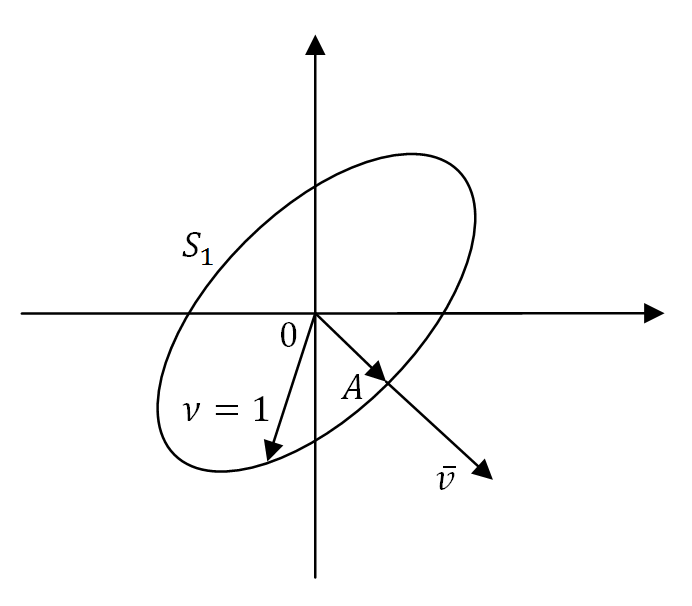
\includegraphics[scale=0.6]{l5_2.png}\\
            $A = $ луч $ \cap S_1$, $~S_1$ --- граница\\
            $\nu(OA) = 1$\\
            $\nu(v) = \lambda \nu(OA) = \lambda$, если $v = \lambda OA, \lambda = \cfrac{|v|}{|OA|}$
        \end{center}
        Покажем, что $B$ -- единичный шар относительно данной нормы. Понятно, что граница луча $A$ лежит в множестве $B$. Поскольку множество ограничено, то луч выходит за множество. Так как множество выпукло и содержит окрестность нуля, то луч пересечёт границу ровно 1 раз. Тогда можно задать на каждом луче единичный вектор $w$, а на каждом противоположном -- вектор $-w$. Так как $B$ центрально симметрично, то $-w$ тоже лежит в $B$. Осталось показать, что $\nu$ -- норма.
        \begin{gather*}
            \forall\ v : \nu(\alpha \cdot v) = \left|\alpha \cdot \dfrac{|w|}{|v|}\right| = |\alpha| \cdot \dfrac{|w|}{|v|} = |\alpha| \cdot \nu(v)\\
            \forall\ v \neq 0 : \nu(v) = \dfrac{|w|}{|v|} > 0\\
            \forall\ v_1,\ v_2 : \nu(v_1 + v_2) = \nu (\alpha \cdot w_1 + \beta \cdot w_2) = |\alpha + \beta| \cdot \nu\left(\dfrac{\alpha}{\alpha + \beta} \cdot w_1 + \dfrac{\beta}{\alpha + \beta} \cdot w_2\right)= \\
            \Downarrow \text{по выпуклости} \Downarrow\\
            = |\alpha + \beta| \cdot \nu (w^*) = |\alpha + \beta| \leqslant |\alpha| + |\beta| = |\alpha| \cdot \nu(w_1) + |\beta| \cdot \nu(w_2) = \nu(v_1) + \nu(v_2)
        \end{gather*}
    \end{enumerate}
    Теперь покажем, что $B$ -- единичный шар относительно некоторой нормы, только если выполняются свойства 1--5. Для этого установим ряд фактов.
    \begin{enumerate}
        \item Любой единичный шар $B$ содержит окрестность нуля.
            
        
        Пусть \[\bar x = \begin{pmatrix}
        x_1 \\
        ...\\
        x_n \\
        \end{pmatrix} = x_1 \bar e_1 +...+x_n \bar e_n \in B_1^{\nu_1} (R = 1)\]
        $\nu_2(\bar x) = \nu_2 (x_1 \bar e_1 +...+x_n \bar e_n) \leqslant \nu_2(x_1e_1)+...+\nu_2(x_ne_n) = |x_1|\nu_2(e_1)+...+|x_n|\nu_2(e_n) \leqslant \\ \leqslant \underset{i=1,...,n}{max} \{\ |x_i|\}$.\begin{center}
            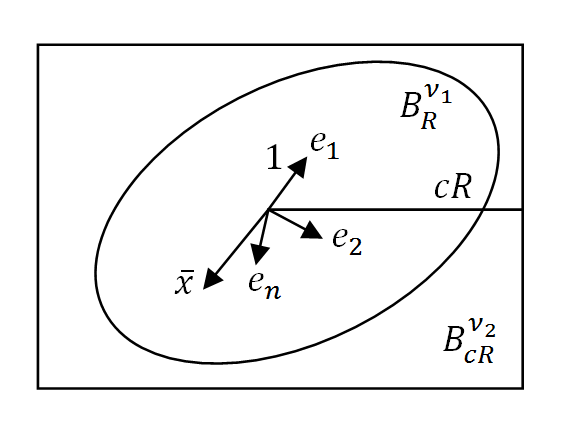
\includegraphics[scale=0.5]{l5_5.png}\end{center}
        Пусть $|\bar x|_{\infty} = \underset{i=1,...,n}{max}|x_i|, ~M = \underset{i=1,...,n}{max}\nu_2(e_i)$, тогда $\nu_2(x) \leqslant |\bar x|_{\infty}nM$, то есть $B_R^{\nu_1} \subset B_{cR}^{|\cdot |_{\infty}}, c = nM$.\\
        Доказали, что любой единичный шар можно поместить в квадрат со стороной $cR$.\\
        \\
        Если $|x|_{\infty} \leqslant \cfrac{1}{nM}$, то $\nu_2(x) \leqslant 1, x \in B_1^{\nu_2}$ откуда и следует требуемое.\begin{center} 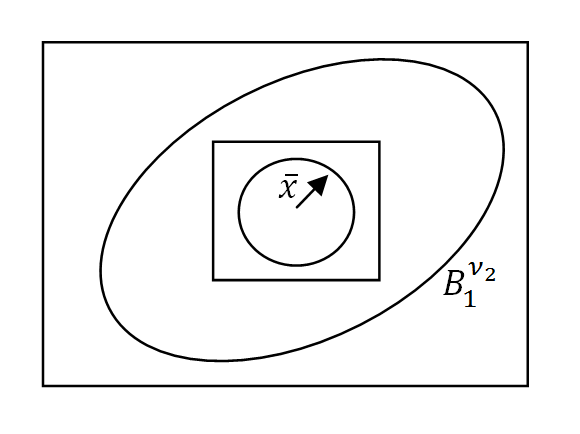
\includegraphics[scale=0.5]{l5_6.png}\end{center}
            
        \item Шар $B$ -- ограниченное и замкнутое множество.
            
        Докажем от противного.\begin{center}$B_1^{\nu} = \{x | \nu(\bar x) \leqslant 1\}$\end{center}
        Рассмотрим $S^2$ -- евклидова сфера $S^{\nu_2}_1 = \{x\mid |x|_2=1\}$. Если множество ограничено и замкнуто, то любая функция на нём достигает максимума и минимума. Покажем, что норма как функция на шаре удовлетворяет такому условию.
                
        Пусть $m = \min\limits_{x \in S} \nu(x)$, тогда при $|x|_2 = 1$ выполнено всегда, что $m \leqslant \nu(x) \iff m \cdot \nu_2(x) \leqslant \nu(x)$. Но если $x \in S$, то $\nu(x) = 1$ и $\nu_2(x) \leqslant \dfrac{1}{m}$, то есть, $S \subset B^{\nu_2}\left(R = \dfrac{1}{m}\right)$. Но тогда и $B \subset B^{\nu_2}\left(R = \dfrac{1}{m}\right)$, следовательно, $B$ -- ограниченное множество.
                
        \begin{center}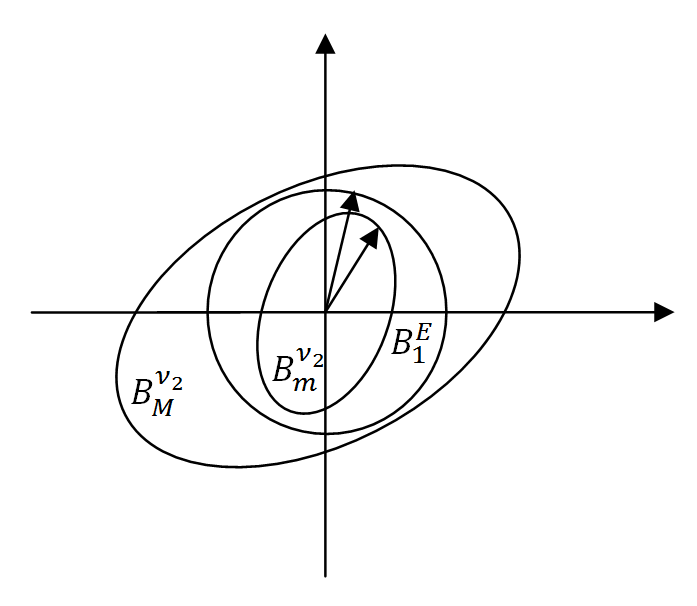
\includegraphics[scale=0.55]{l5_7.png}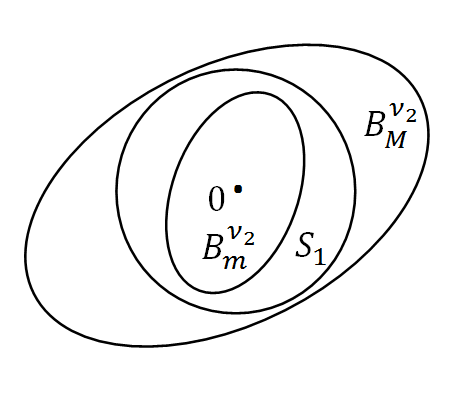
\includegraphics[scale=0.55]{l5_9.png}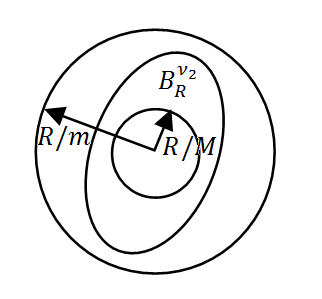
\includegraphics[scale=0.65]{l5_8.png}\end{center}
        
        Теперь покажем, что $B$ замкнуто. Для этого установим непрерывность нормы.
        
        $\textbf{Лемма}$. Норма $\nu : \mathbb{R}^n \to \mathbb{R}^n$ непрерывна.
        
        Докажем определение непрерывности для нормы: 
        \[\forall\ \varepsilon > 0 \exists\ \delta > 0 \mid |x - x_0|_2 < \delta \Rightarrow |\nu(x) - \nu(x_0)| < \varepsilon\]
        Положим $\delta = \dfrac{1}{M \cdot n} \cdot \varepsilon$, где $M$ и $n$ мы взяли те же, что и в пункте про окрестность нуля. Тогда $B_{x_0}^{\nu_2}\left(\dfrac{1}{M \cdot n}\right) \subset B_{x_0}^{\nu}(1)$ (шар содержит окрестность нуля), откуда $B_{x_0}^{\nu_2}\left(\dfrac{\varepsilon}{M \cdot n}\right) \subset B_{x_0}^{\nu}(\varepsilon)$. Тогда:
        \[|x - x_0|_2 < \delta \Longrightarrow \nu(x - x_0) < \varepsilon\]
        Теперь, воспользовавшись свойствами нормы, получаем требуемое:
        \begin{gather*}
            \nu(x) = \nu(x - x_0 + x_0) \leqslant \nu(x - x_0) + \nu(x_0) \leqslant \varepsilon + \nu(x_0)\\
            \nu(x_0) = \nu(x_0 - x + x) \leqslant \nu(x_0 - x) + \nu(x) < \varepsilon + \nu(x)\\
            -\varepsilon < \nu(x) - \nu(x_0) < \varepsilon \\
            |\nu(x) - \nu(x_0)| < \varepsilon
        \end{gather*}
        Докажем теперь замкнутость шара. Так как $\nu$ непрерывна, то 
        \[\forall\ \varepsilon > 0\ \exists\ x_\varepsilon \neq x_0 \mid x_\varepsilon \in B \cap \cup_\varepsilon(x_0)\]
        Но это означает, что $\nu(x_0) = \displaystyle\lim\limits_{\varepsilon \to 0} \nu(x_\varepsilon) \leqslant 1$, так как $\nu(x_\varepsilon) \leqslant 1$. Следовательно, предельная точка также содержится в единичном шаре $B$.  А это ни что иное, как определение замкнутости.
        \item Любой шар $B$ радиуса $R$ -- выпуклое множество.
        
        Пусть $x \in B,\ y \in B$. Тогда $\nu(x) \leqslant R$,\ $\nu(y) \leqslant R$. Пусть $z = t \cdot x + (1 - t) \cdot y$ -- точка, являющаяся выпуклой комбинацией $x$ и $y$. Тогда:
        \[\nu(z) = \nu(t \cdot x + (1 - t) \cdot y) \leqslant \nu(t \cdot x) + \nu\big((1 - t) \cdot y\big) = t \cdot \nu (x) + (1 - t) \cdot \nu(y) \leqslant t \cdot R + (1 - t) \cdot R = R\]
        
        \item Любой шар центрально симметричен
        
        Пусть $x \in B \Rightarrow \nu(x) \leqslant R$. В то же время, в силу свойств нормы:
        \[-x = (-1) \cdot x \Rightarrow \nu(-x) = |-1| \cdot \nu(x) \leqslant R\] 
            
        \end{enumerate}
        
        Из доказанных выше утверждений напрямую следует факт, что $B$ -- единичный шар относительно нормы $\nu$, если и только если выполнены вышеуказанные свойства.
    
\end{proof}
\textbf{Пример 1.}\\
$B = \{x^2+axy+4y^2 \leqslant 1\}$\\
Существует ли такая норма $\nu$, что $B$ --- единичный шар относительно нее ($B = B_1^{\nu}$)?\\
\begin{center}
    $
    \begin{pmatrix}
    1 & \cfrac{a}{2}\\
    \cfrac{a}{2} & 4
    \end{pmatrix}
    $
    \\ ~\\
    $\vartriangle_1 = 1 > 0$\\
    $\vartriangle_2 = 4 - \cfrac{a^2}{4} > 0$\end{center}
То есть это эллипс, все 5 свойств из предыдущей теоремы выполняются, значит при $|a| < 4 B$ --- единичный шар относительно нормы.\begin{center}
    $\vartriangle_1 = 1 > 0$\\
    $\vartriangle_2 = 4 - \cfrac{a^2}{4} < 0$\end{center}
В этом случае множество не будет замкнутым, то есть не выполняются все свойства из предыдущей теоремы, значит в этом случае $B$ не будет единичным шаром относительно нормы.\\
При $\vartriangle_2 = 0$: $ a = \pm 4$ и $x^2 \pm 4xy+4y^2 \leqslant 1$, $(x \pm 2y)^2 \leqslant 1$. В этом случа получим множество между двумя параллельными прямыми, которое является незамкнутым, то есть в этом случае $B$ тоже не будет единичным шаром относительно нормы.\\
Получили, что $B = B_1^{\nu}$ только при $|a| < 4$.
\subsection{Скалярное произведение}
\begin{definition}
$V$ --- \textbf{евклидово пространство со скалярным произведением}, если задана $V \times V \rightarrow \mathbb{R}$, то есть, на нем задано скалярное произведение $(\bar u, \bar v) \in \mathbb{R}$ такое, что для пространств над $\mathbb{R}$ выполнено:\begin{enumerate}
    \item $(u, v) = (v, u)$
    \item $(u'+u'', v) = (u', v)+(u'', v)$
    \item $\alpha (u, v) = (\alpha u, v) = (u, \alpha v), \alpha \in \mathbb{R}$
    \item $(u, u) > 0, u \neq \bar 0~ ((u, u) = 0 \Leftrightarrow u=0)$
\end{enumerate}
Обозначение скалярного произведения: $(u, v)=<u, v>=<u~|~v>$.
\end{definition}
\begin{proposal}
Длина вектора --- это $|v| = \sqrt{(v, v)} \geqslant 0$ (норма).
\end{proposal}
\begin{proof}
\ 	
\begin{center}$|\alpha v| = \sqrt{(\alpha v, \alpha v)} = \sqrt{\alpha^2 (v, v)} = |\alpha||v|$\\
    $|v| > 0$, при $v \neq \bar 0$\\
    $|u+v| \leqslant |u|+|v|$\end{center}

\end{proof}
$$cos \widehat{(u, v)} = \cfrac{(u, v)}{|u||v|}, u, v \neq \bar 0$$
\begin{definition}
$V$ --- \textbf{эрмитово пространство со скалярным произведением}, если задана $V \times V$ $\rightarrow \mathbb{C}$, то есть, на нем задано скалярное произведение $(\bar u, \bar v) \in \mathbb{C}$ такое, что для пространств над $\mathbb{C}$ выполнено:\begin{enumerate}
    \item $(u, v) = \overline{(v, u)}$
    \item $(u'+u'', v) = (u', v)+(u'', v)$
    \item $\alpha (u, v) = (\alpha u, v) = (u, \alpha v), \alpha \in \mathbb{C}$
    \item $\forall u~ (u, u) \geqslant 0, (u, u) = 0 \Leftrightarrow u=0$
\end{enumerate}
\end{definition}
Как по норме $|w|$ восстановить скалярное произведение $(u, v)$?
\begin{center}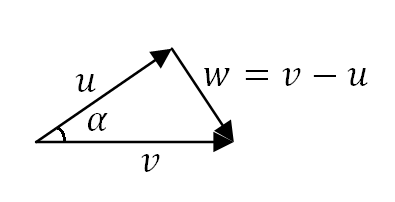
\includegraphics[scale=0.55]{l5_10.png}\\
    $|w|^2 = (w, w) = (v-u, v-u) = (v, v) - (u, v) - (v, u) + (u, u) = |v|^2 - 2(u, v) + |u|^2$\end{center}
То есть, $(u, v) = \cfrac{1}{2}(|v|^2 + |u|^2 - |v-u|^2)$.\\
\\
\begin{theorem}[Тождество параллелограмма]
Пусть $V$ --- нормированное пространство с нормой $|v|$. На $V$ существует такое скалярное произведение, что $|v| = \sqrt{(v, v)}$ в том и только том случае, когда в $V$ выполняется тождество параллелограмма:\begin{center}
    $\forall a, b~ |a+b|^2 + |b-a|^2 = 2(|a|^2 + |b|^2)$\end{center}
При $c = a+b, d = b-a:$ \begin{center}$c^2+d^2 = 2(a^2+b^2)$\\
    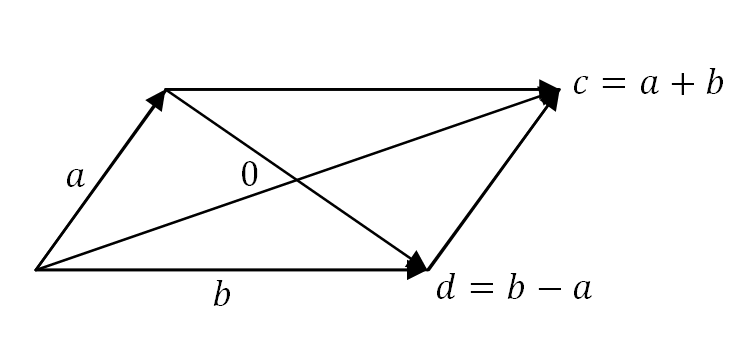
\includegraphics[scale=0.55]{l5_11.png}\end{center}
\end{theorem}
\begin{proof}
Если для $\forall v ~|v| = \sqrt{<v, v>}$, то $|a+b|^2+|b-a|^2 = <a+b, a+b> + <b-a, b-a> = \\=<a, a> + 2<a, b> + <b, b> +<b, b> - 2<a, b> + <a, a> = 2(|a|^2 + |b|^2)$
\end{proof}
\subsection{Ортогональные системы}
\begin{definition}
$H$ --- \textbf{гильбертово пространство}, если на нем задано скалярное произведение и оно является полным (относительно метрики, порожденной скалярным произведением).\end{definition}
\begin{definition}
Набор $\{ \varphi_0, \varphi_1,...,\varphi_n,...\}^{-e}$ называется \textbf{ортогональной системой}, если \\$(\varphi_i, \varphi_j) = \delta_j^i = 
\left\{  
\begin{array}{lcl}  
1, i = j \\  
0, i \neq j \\
\end{array}   
\right.  
$
\end{definition}
Формально хотим представить $f = \sum\limits_{n=0}^{\infty} c_n \varphi_n$.\begin{center}
    $(f, \varphi_j) = c_j(\varphi_j, \varphi_j)$\\ 
    $(\varphi_j, \varphi_j) = 1$\\ 
    $c_j = \cfrac{(f, \varphi_j)}{\parallel \varphi_j \parallel^2} = (f, \varphi_j)$\end{center} $c_j$ --- коэффициенты Фурье по ортогональной системе.\\ \\
\begin{theorem}
Если $\varphi_j$ --- ортогональная система, тогда следующие условия эквивалентны:\begin{enumerate}
    \item система $\{\varphi_j\}$ является базисом, то есть $f = \sum\limits_{n=0}^{\infty}c_n \varphi_n$
    \item выполнение равенства Парсеваля $\parallel f \parallel^2 = \sum\limits_{n=0}^{\infty}c_k^2$
    \item система является полной, то есть $\exists y \neq 0: (\varphi_j, y) = 0$
\end{enumerate}
\end{theorem}
Хотим приблизить $f$ и минимизировать $\parallel f - \sum\limits_{k=0}^n \alpha_k \varphi_k \parallel \to min$.\\
$(f - \sum\limits_{k=0}^n \alpha_k \varphi_k, f - \sum\limits_{k=0}^n \alpha_k \varphi_k) =$ (так как система ортогональна) $= (f, f) - 2\sum\limits_{k=0}^n \alpha_k (f, \varphi_k) +\\+\sum\limits_{k=0}^n \alpha_k^2 (\varphi_k, \varphi_k) = (c_k=(f, \varphi_k),~ (\varphi_k, \varphi_k)=1) = \parallel f \parallel^2 + \sum\limits_{k=0}^n (\alpha_k - c_k)^2 - \sum\limits_{k=0}^n c_k^2$\\
Выбором $\alpha$ хотим минимизировать, минимальная норма будет там, где совпадают $\alpha_k = c_k$.\\
\\
$a = \{1, x, x^2,..., x^n\}$ --- пространство $\mathbb{R}_{n+1}$ многочленов степени $\leqslant n$ на $[-1, 1]$, где скалярное произведение $\int\limits_{-1}^1 f(x)g(x)\,dx$. Применим к $a$ процесс Грама-Шмидта, получим $b$.\begin{center}
    $a \to b = \{P_0(x)=1\}$\end{center}
\begin{definition}
\textbf{Многочленами Лежандра} называются многочлены вида:
\begin{center}$P_k(x) = \cfrac{1}{2^k k!}\cfrac{d^k}{dx^k}((x^2-1)^k)^{(k)}, k=1,..,n$\end{center}\begin{description} 
    \item[k=0:] $P_0(x)=1$
    \item[k=1:] $P_1(x)=\cfrac{1}{2}(x^2-1)'=x$
    \item[k=2:] $P_2(x)=\cfrac{1}{8}((x^2-1)^2)''=\cfrac{1}{8}(4x(x^2-1)'=\cfrac{3x^2-1}{2}$
    \item[k=3:] $P_3(x)=\cfrac{1}{48}((x^2-1)^3)'''=\cfrac{1}{2}(5x^3-3x)$\end{description}
$\parallel P_1(x) \parallel = \sqrt{\int\limits_{-1}^1 x \cdot x\,dx} = \sqrt{\cfrac{2}{3}}$
\end{definition}
\subsection{Домашнее задание 5}\begin{enumerate}
    \item
    \begin{enumerate}
        \item Проверить ортогональность $P_2(x)$ и $P_3(x)$ относительно $<f, g> =\\= \int\limits_{-1}^1 f(x)g(x)\,dx$.
        \item Найти $\parallel P_n(x) \parallel$.
    \end{enumerate}
    \item
    Найти $\alpha_0, \alpha_1, \alpha_2$ на $[-1, 1]$: $\parallel f - \sum\limits_{k=0}^2 \alpha_kP_k(x) \parallel \to min$, $d_j=\cfrac{(f, \varphi_j)}{\parallel \varphi_j \parallel^2} = (f, \varphi_j)$, где $P_k(x)=\cfrac{1}{2^k k!}\cfrac{d^k}{dx^k}((x^2-1)^k)^{(k)},~k=1,\cdots, n$ --- многочлены Лежандра.
    \begin{enumerate}
        \item $f_1(x)=xe^{-x}$
        \item $f_2(x)=x^3$\\
    \end{enumerate}
    \item
    Выразить скалярное произведение через длину вектора в эрмитовом пространстве.\end{enumerate}